\scanpage{80}
% archive foliation: 79
$\omega$ base de $\underline\omega^{\otimes n}$ $(n\in\mathbf Z,n\ne0)$

$\omega^{1/n}$ base de $\underline\omega$ définie loc. \unsure{mod} mult.
par $\varepsilon$, $\varepsilon^n=1$

$\int\omega^{1/n}$ bien défini mod transformations
$f\longmapsto\varepsilon f+b$ $(\unsure{\varepsilon^n=1|\varepsilon\equiv1})$
\inserted{donc $c_{\int\omega^{1/n}}$ bien défini}

Si $t$ uniformisante et $\omega=f(t)dt^n$, on aura
\[
\omega^{1/n}=f^{1/n}dt\quad\text{et}\quad
\deleted{\unsure{c_{\int\omega^{1/n}}}}
c_{\int\omega^{1/n}}=c_{\int f^{1/n}dt}\deleted{=c_t+}
\]
\[
c_n(\omega)=c_t+\left[-\frac2n\frac{f''}{f}
+\frac{2n+1}{n^2}\left(\frac{f'}f\right)^2\right]dt^2
\qquad\text{si }n\ne0
\]

\deleted{$\unsure{Gc_n(\omega)}$}
\[
\begin{aligned}
G_{m,n}\left(
\underset{\substack{\Vert\\f(dt)^m}}{\omega_m},
\underset{\substack{\Vert\\g(dt)^n}}{\unsure{\omega'_n|\omega_n}}\right)
&=c_n(\unsure{\omega'_n|\omega_n})-c_m(\omega_m)\\
&=\left[\left(-\frac2n\frac{g''}{g}
+\frac{2n+1}{n^2}\left(\frac{g'}g\right)^2\right)\right.\\
&\unsure{-}\qquad\left.-\left(-\frac2m\frac{f''}f
+\frac{2m+1}{m^2}\left(\frac{g'}g\right)^2\right)\right]dt^2
\end{aligned}
\]
\[
\left\{\begin{aligned}
G_{m,n}(\omega_m,\omega'_n)+G_{n,\unsure{r|p}}(\omega'_n,\omega''_p)
&=G_{m,p}(\omega_m,\omega''_p)\\
G_{m,n}(\omega_m,\omega_n)&=G_{m,nr}(\omega_m,\omega_n^r)
\quad\text{si }n\ne0,\ r\ne0\\
G_{m,n}(\omega_m,ds)&=G_{m,0}(\omega_m,s)\\
G_{0,0}(t,s)&=G(t,s)
\end{aligned}\right.
\]
\inserted{\[
G_{m,n}(\omega_m,(ds)^n)=G_{m,0}(\omega_m,s)
\]}
\figure{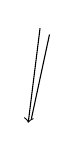
\begin{tikzpicture}[x=1cm,y=1cm]
\draw[->] (0.15,1.2)--(0,0);\draw (0.27,1.12)--(0.04,0.05);
\end{tikzpicture}}
\[
G_{m,n}((dt)^m,(ds)^n)=G_{0,0}(t,s)
\]
\margin{$c'_n(\omega)=n^2\dfrac{c_n(\omega)}{\deleted{\unsure{12}}}
\in\mathcal T_X^{\unsure{\otimes|*}n^2}$}

\deleted{$c'_n(\omega)$}\qquad $m,n\qquad
\delta=m\alpha=n\beta\qquad\delta^2=m^2\alpha^2=n^2\beta^2$
\[
\begin{aligned}
\omega_m\longmapsto{}&\alpha^2\deleted{\unsure{c}}c'_m(\omega_m)
=\alpha^2m^2\frac{c_m(\omega_m)}{12}
\deleted{\unsure{\in\Gamma\mathcal T_X^{\otimes\delta^2}}}\\
&=\frac{\delta^2c_m(\omega_m)}{12}
\in\Gamma\mathcal T_X^{\unsure{\otimes|*}\delta^2}
\end{aligned}
\]
\[
\omega'_n\unsure{\mathrel{\mid\!\!-\!\!-}|\longmapsto}
\beta^2c'_n(\omega'_n)
=\beta^2n^2\frac{c_n(\omega'_n)}{12}
=\delta^2\frac{c_n(\omega'_n)}{12}
\in\Gamma\mathcal T_X^{\unsure{\otimes|*}\delta^2}
\]
\[
G'_{m,n}(\omega_m,\omega'_n)=\alpha^2c'_m(\omega_m)-\beta^2c'_n(\omega'_n)
\in\Gamma\mathcal T_X^{\unsure{\otimes|*}\delta^2}
\]
\[
\left\{\begin{aligned}
\unsure{G_n|G}(t,as)&=G(t,s)&a&\in\Gamma(S,\mathcal O_S^*)\\
G(t,s+b)&=G(t,s)&b&\in\Gamma(S,\mathcal O_S)\\
G(t,1/s)&=G(t,s)&s&\in\operatorname{Et}_S(X,G_{m,S})
\end{aligned}\right.
\]

% The following calculations are written upside down at the foot and lower right.
\margin{\[
\begin{gathered}
f\longmapsto af+b\qquad df=dg\Longrightarrow G(f,g)=0\\
f\longmapsto af\qquad
\left(\frac{df}{f}\right)^2=\left(\frac{dg}{g}\right)^2
\Longrightarrow G(f,g)=0\\
df\qquad\left(\frac{df}{f}\right)^2\qquad
(df-dg)\left(\left(\frac{df}{f}\right)^2-
\left(\frac{dg}{g}\right)^2\right)\\
\frac{df}{f}=c\frac{dg}{g}\qquad ?\\
\log f=c\log g\\
f=g^c
\end{gathered}
\]}
\figure{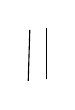
\begin{tikzpicture}[x=1cm,y=1cm]
\draw (0,0)--(0.02,0.65);\draw (0.23,0.02)--(0.23,0.67);
\end{tikzpicture}}

